\section{Roofline}
\label[appendix]{sec:roofline}

The roofline model used in this document was prepared according to the guidelines in \cite{williams08}, except for the memory bandwidth roof and some adaptations. Compared to operational intensity, computational intensity (or arithmetic intensity) is a more complete measure for the program studied in this document.

As stated in \cref{sec:env}, the roofline model presented in this document refers to a very specific node of SeARCH Group 201.

According to \cite{xeon5100,intelsys,inteloptimize}, these nodes' micro architecture is \intel Core\texttrademark, which is capable of decoding up to five instructions per cycle, has a throughput of up to 4 instructions per cycle and three full arithmetic logical units, where each has a throughput of one instruction per cycle for many kinds of computational instructions. This binds the peak throughput of computational instructions at 3 per cycle.

Since each core has a peak throughput of 3 computational instructions per cycle, each processor has 2 cores at a clock frequency of 2.0 GHz, and each node has 2 processors, this results in a peak of
\begin{IEEEeqnarray}{rCl}
3\times 2\times 2\times 10^{9}\times 2 & = & 24\;\mathrm{GInstructions/s}\enspace .
\end{IEEEeqnarray}
This value corresponds to the CPU roof.

Although \cite{williams08} recommends using ``a series of highly tuned versions of the STREAM benchmark'', the creation of such versions is out of the scope of this project. As such, the peak memory bandwidth was measured running the original STREAM benchmark in a SeARCH Group 201 node. The benchmark returned a peak value of 4.78 GB/s, which is the memory roof.

As for CPU ceilings, these were calculated decreasing the number of cores used, first by using only one processor (half the peak), then by removing thread-level parallelism (one core, a quarter of the peak). As measured in the previous report, this algorithm already presents itself with a high balance of floating-point multiplications and additions (two thirds of the TLP ceiling, as one of the ALUs would remain idle). The last CPU ceiling remaining would mean removing all the instruction-level parallelism (half the Mul/Add balance ceiling, only one ALU active).

Lastly, the absence of dual channel was used as the only memory ceiling. The influence of any other mechanism such as prefetch or unit stride accesses would have to be properly measured with the recommended tuned versions, which are not available for this document.

\Cref{fig:roofline} shows the resulting roofline model for the nodes of SeARCH Group 201.

\begin{figure}[!htp]
	\begin{center}
		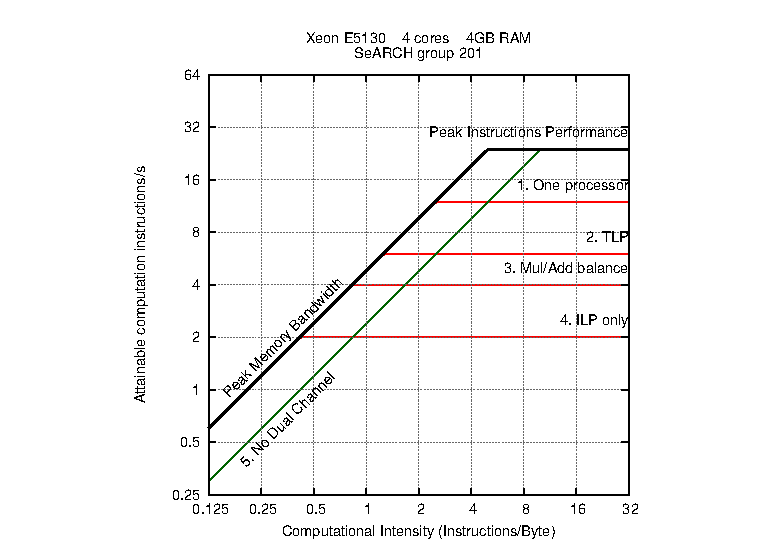
\includegraphics[width=\columnwidth]{images/roofline201}
	\end{center}
	\caption{Roofline for SeARCH Group 201.}
	\label{fig:roofline}
\end{figure}
